\documentclass{article}
\usepackage{polski}
\usepackage[utf8]{inputenc}
\usepackage{graphicx}
\usepackage[export]{adjustbox}
\usepackage{listings}
\usepackage{xcolor}
\lstset{ %
  backgroundcolor=\color{white},
  basicstyle=\footnotesize,
  breakatwhitespace=true,
  breaklines=true,
  captionpos=b,
  extendedchars=true,
  frame=single,
  keepspaces=true,
  keywordstyle=\color{blue},
  language=C++,
  morekeywords={*,...},
  numbers=left,
  numbersep=5pt,
  numberstyle=\tiny\color{gray},
  rulecolor=\color{black},
  showspaces=false,
  showstringspaces=false,
  showtabs=false,
  stepnumber=1,
  tabsize=4
}

\title{Symulacja "galaktyki"}
\author{Filip Piórski [REDACTED] Programowanie Obiektowe \(PROE\) prowadzący [REDACTED]}
\date{\today}

\begin{document}

\maketitle
\vspace{1cm}

\section{Abstrakt}
Program symuluje układ dowolnej ilości ciał niebieskich przybliżonych przez punktowe masy. Program został napisany w duchu OOP, w związku z czym jego działanie opiera się o istnienie klas i polimorfizmu.
\newpage
\section{Diagram w UML}
\begin{center}
\vspace{5mm}
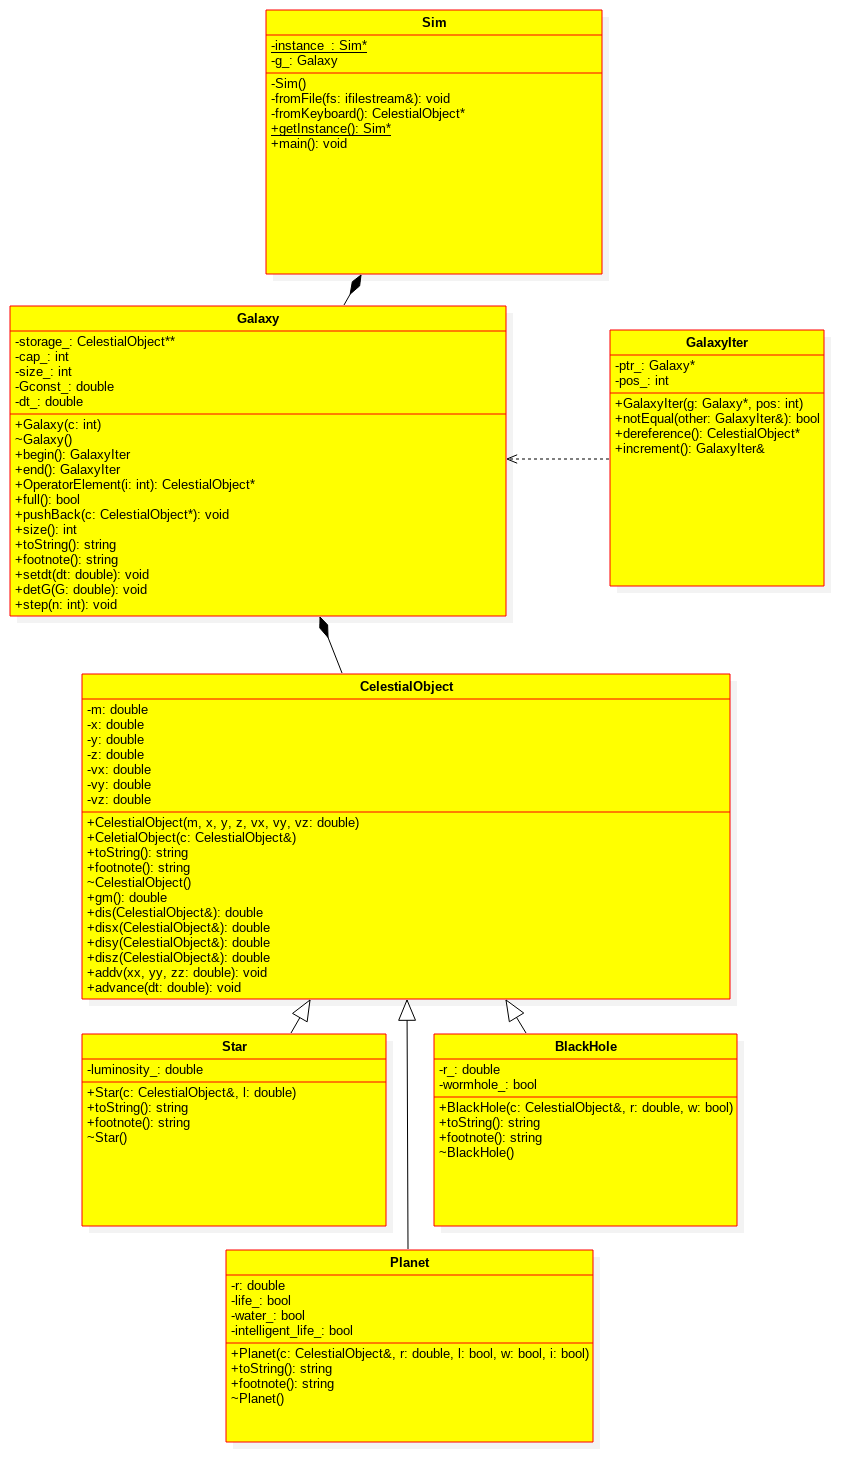
\includegraphics[height=17cm]{UML}
Nie byłem pewny co do tego jaka jest UMLowska zależność pomiędzy iteratorem klasy Galaxy a samą klasą, więc zdecydowałem się na zależność
\newpage

\section{Opis klas}
\subsection{Sim}
Główna klasa, realizuje wzorzec singleton, jako jedyna komunikuje się ze światem zewnętrznym
Zawiera całą część sterującą programu
\subsection{Galaxy oraz GalaxyIter}
GalaxyIter jest klasą pomocniczą, wymaganą aby móc wykorzystać ranged fory z C++11
Galaxy to kolekcja wskaźników na CelestialObject, działa jak mocno uproszczona wersja std::vector<CelestialObject*> oraz zawiera parametry symulacji wspólne dla wszystkich
Jej metody toString\(\) oraz footnote\(\) stanowią interfejs łączący Sim z CelestialObject - Galaxy wywołuje odpowiednie metody każdego z przechowywanych przez nią CelestialObject po czym łączy je razem oraz dodaje parametry wspólne od siebie zaraz przed odesłaniem wyniku do wywołującego metodę singletonu.
\subsection{CelestialObject oraz klasy dziedziczące}
CelestialObject to klasa bazowa która ma cechy wspólne większości ciał niebieskich - masę, położenie oraz prędkość
Klasy dziedziczące po niej to Star, Planet oraz BlackHole, każda z dodatkowymi własnymi parametrami.
Polimorfizm został użyty przy dwóch metodach - toString\(\) oraz footnote\(\), które są wirtualne w klasie bazowej i nadpisane w klasach pochodnych, więc kiedy Galaxy wywołuje metodę przy użyciu wskaźnika na CelestialObject wywoływana jest odpowiednia metoda klasy pochodnej
\section{Opis użycia programu}
Program korzysta z minimalnej biblioteki linenoise \(informacje licencyjne - plik linenoise_LICENCE\) do komunikacji z użytkownikiem aby była ona wygodniejsza niż klasyczne wczytywanie ze strumienia wejściowego oraz bardziej przypominała korzystaine z UNIXowego terminala. Do programu dołączona jest także bardzo skromna aczkolwiek pomocna komenda help, która powinna rozjaśnić jakiego rodzaju wejścia oczekuje program.
Dołączony jest plik ex1.txt, po wczytaniu którego w pamięci programu powinny się znaleźć dwa ciała niebieskie - gwiazda oraz planeta ją orbitująca. Wpisując komendę "step" z parametrem z zakresu 1000-10000 powinno udać się zaobserwować ruch kołowy patrząc na współrzędne planety.
\subsection{Kompilacja}
Program kompiluje się przy użyciu skryptu Scons, komendą "scons"
\newpage
\section{Dowód działania programu}
\begin{center}
\vspace{5mm}
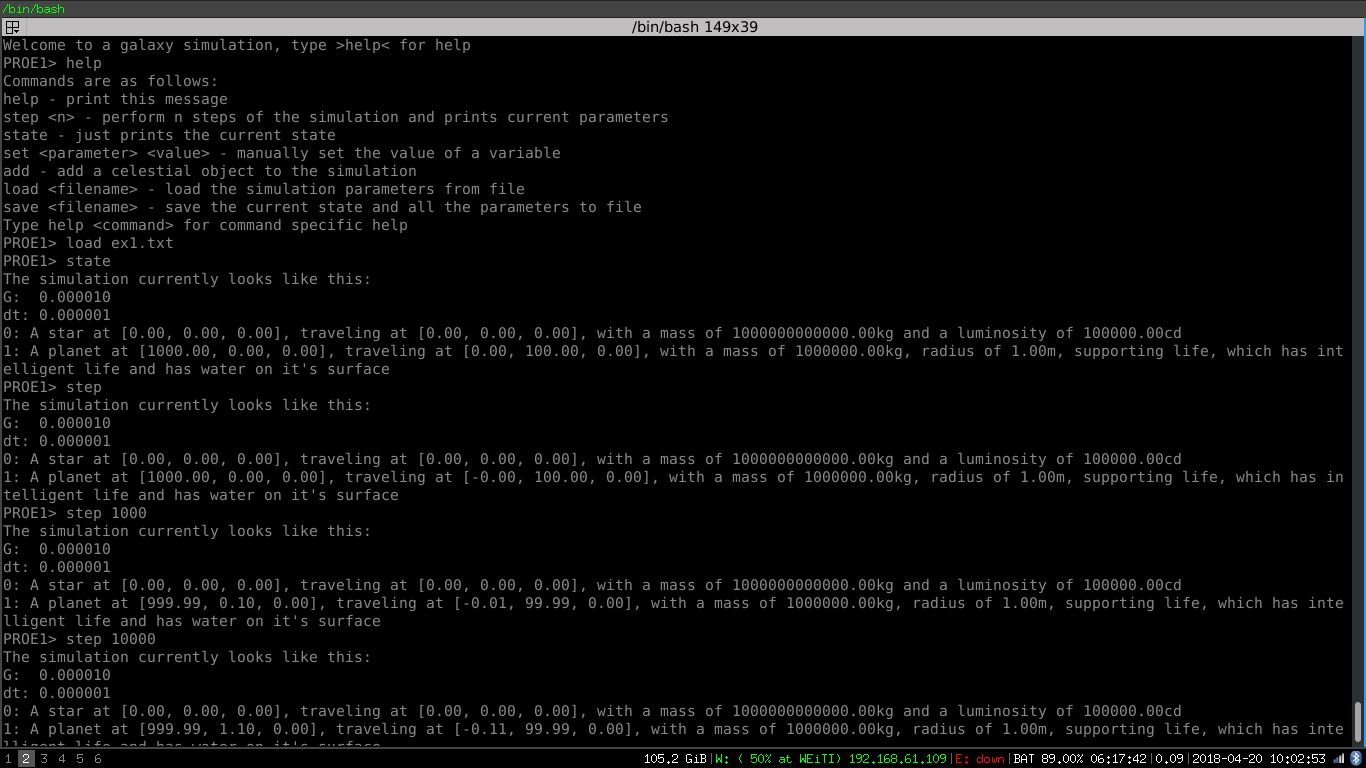
\includegraphics[height=9cm]{dowod1}\\
\newpage
